\chapter[АНАЛИТИЧЕСКИЙ ОБЗОР ЛИТЕРАТУРЫ]{АНАЛИТИЧЕСКИЙ ОБЗОР \\ ЛИТЕРАТУРЫ}

Информатикс -- важная часть экосистемы Российского олимпиадного программирования.
Ресурс используется при подготовке учеников к различным олимпиадам,
а так а так же для проведения уроков информатики в Российских школах.

Информатикс был создан в 2007 году и имеет более чем 10-летнюю историю.
Сайт имеет огромную базу задач, более 6 тысяч, 
что делает его одной из крупнейших русскоязычных баз задач по программированию, в которой накоплены материалы проводившихся за многие годы олимпиадных мероприятий. 
Стоимость базы задач Информатикс быда оценена экспетами примерно в 60 миллионов рублей. 

В то же время, на большую часть задач распространиются различные копирайт-условия, разрешающие их использование только на ресурсе Информатикс.

Помимо этого, важной частью Информатикс является контент курсов и уроков, 
который также был накоплен за годы существования ресурса.

Также Информатикс используется для различных сборов, например, Летняя Олимпиадная Школа (ЛОШ), 
и для проведения различных отборов, например, отбор в Образовательный центр "Сириус" по дисциплине программирование\cite{inf_tinkoff}.

Информатикс также используется в целях самоподготовки.
Ученики могут найти контест, использовавшийся в каком либо соревновании и отборе и самостоятельно решить его.
Также они могут найти и отдельную задачу из базы Информатикс и решить её отдельно.

Отдельной ценностью является база посылок, где хранится более 15 миллионов протестированных исходных кодов решения задач -- посылок --, их результатов и протоколов тестирования. 

Стоит также отметить, что Информатикс принадлежит организации ГБОУ ЦПМ, что расшифровывается как Центр Педогагической Подготовки,
и бюджет организации имеет серьёзное органичение на ресурсы, выделяемые на аренду и покупку аппаратных мощностей.

Так же важным требованием к системе можно считать необходимость практически полной доступности сайта (Доступность сайта должна стремиться к 100\%), 
а все технические работы проходить без простоев основной функциональности сайта.

Количество пользователей Информатикс растёт каждый год примерно на 20 \%. 
Иллюстрация \ref{fig:people_count} демонстрирует рост количества пользователей.

\begin{figure}
  \centering
  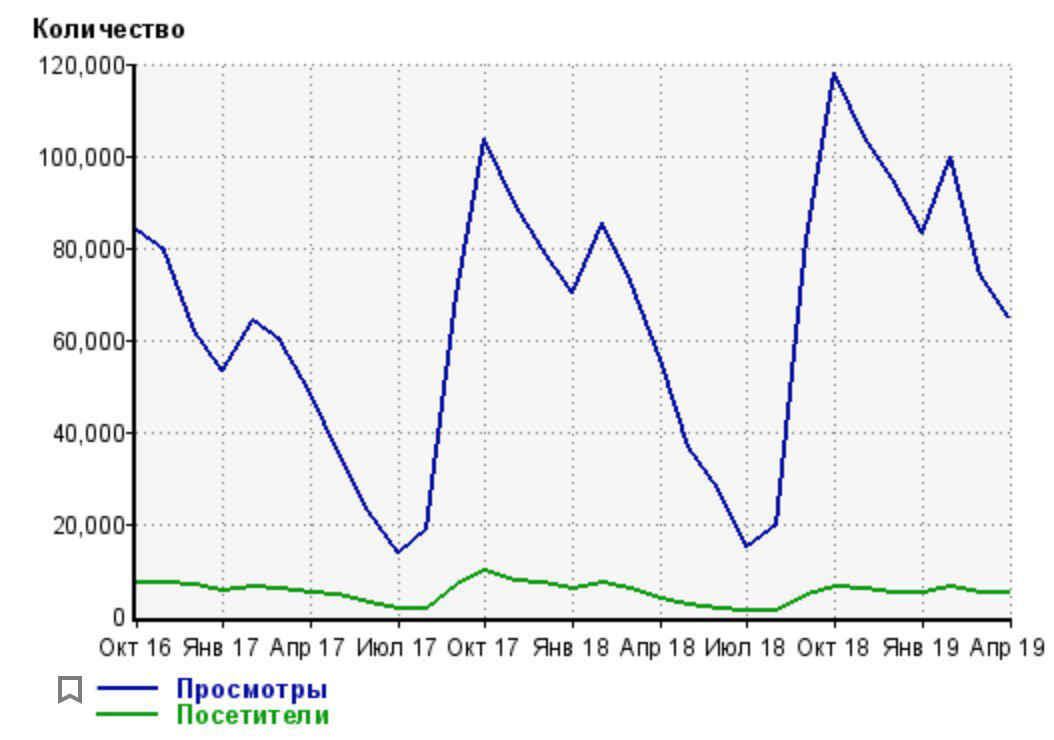
\includegraphics[width=\textwidth]{figures/pepole_count.png}
  \caption{Количество просмотренных страниц на Информатикс по дням с апреля 2016 года по апрель 2019.}
  \label{fig:people_count}
\end{figure}

Помимо вышесказанного, существует потенциал Информатикс для использования его как базы задач и систему тестирования в сторонних проектах и системах.

\section{Существующие аналоги}

Аналогами Информатикс с точки зрения проведения контестов
-- соревнований по спортивному программированию -- 
можно считать ресурсы Codeforces, Яндекс.Контест и другие.

Однако ресурс Яндекс.Контест не предоставляет возможностей для самостоятельного прохождения контестов -- после окончания регистрации на соревнование порешать контест уже не получится.

Также Яндекс.Контест не предоставляет возможности решать задачи не в рамках контеста.
Помимо этого, ресурс был создан компанией Яндекс в своих утилитарных целях,
и политика ресурса не даёт возможности свободно создавать свои задачи
и проводить свои контесты, как это можно делать на Информатикс.

Codeforces -- российский сайт олимпиадного программирования, известный и за рубежом\cite{codeforces_countries}.
Codeforces в отличие от Яндекс.Контест предоставляет возможности по самостоятельной подготовке в рамках решения отдельных задач, однако нельзя решить целый контест.

Также стоит отметить, что Codeforces -- частная компания, 
и для создания и проведения контеста может потребоваться заплатить.
В то же время, Информатикс совершенно бесплатен для своих пользователей.

Аналогами Информатикс с точки зрения базы олимпиадных задач 
можно считать ресурсы Codeforces и Timus Online Judge (или просто Тимус).
Codeforces уже был рассмотрен выше.

Timus Online Judge -- это крупнейший в России архив задач по программированию с автоматической проверяющей системой. Основной источник задач для архива — соревнования Уральского федерального университета, Чемпионаты Урала, Уральские четвертьфиналы ICPC, Петрозаводские сборы по программированию\cite{timus_main}.

Тимус предоставляет возможность решать отдельные олимпиадные задачи.
Однако эти задачи, в отличие от Информатикс, не сгруппированны в контесты.

С точки зрения LMS у Информатикс так же есть аналоги, начиная от Moodle, 
на котором базируется и сам Информатикс (подробнее см. главу \ref{lab:inf_moodle}),
Canvas и OpenEDX, однако очевидно, что данные системы не имеют специфичного для олимпиадного программирования функционала, такого, как автоматическая проверка задач по программированию и другого.

Сводная информация, сравнивающая Информатикс и другие ресурсы, представлена в таблице \ref{tab:inf_and_oth}.

\begin{center}
  \begin{longtable}{|p{0.3\textwidth}|p{0.20\textwidth}|p{0.1\textwidth}|p{0.1\textwidth}|p{0.2\textwidth}|}
    \caption{Сравнение Информатикс и аналогов}
    \label{tab:inf_and_oth}
    \\ \hline
    Характеристика & Codeforces & Timus & Canvas & Информатикс \\
    \hline \endfirsthead
    \subcaption{Продолжение таблицы~\ref{tab:inf_and_oth}}
    \\ \hline \endhead
    \hline \subcaption{Продолжение на след. стр.}
    \endfoot
    \hline \endlastfoot
    Решение задач по программированию & Есть & Есть & Нет & Есть \\
    \hline
    Контесты & Нет & Нет & Есть, как уроки & Есть \\
    \hline
    Функционал LMS & Нет & Нет & Нет & Есть \\
    \hline
  \end{longtable}
\end{center}

Таким образом, можно сделать вывод о том, что полных аналогов Информатикс не существует.

\section{Проблемы Информатикс}

Основная жалоба пользователей на Информатикс -- постоянные сообщения об ошибке отправки задачи:
при сколько-нибудь значительном мероприятии, проводимом на Информатикс (например, одновременно 100 учеников), система перестаёт стабильно принимать посылки и отклоняет их с ошибкой\cite{inf_not_working}. 
Это мешало как простым пользователям-ученикам 
(кейс ученик на уроке информатики в школе пытается сдать задачу, и, хоть он её решил, у него не получается этого сделать), 
так и пользователям, участующем в мероприятии, так как обычно такие мероприятия имеют ограничения во времени.

С точки зрения создателей курса и пользователей LMS (далее -- учителей),
у сайта были проблемы с отображением результатов тестирования (далее -- мониторов).

Мониторы -- отображение количества решённых учеником задач в различных контестах, собранное в единую таблицу.

Мониторы работали очень медленно, а если количество результатов было достаточно большим 
(например, более 50 задач в контесте и более сотни учеников), 
не работали вообще (как было выяснено позднее, они специально были отключены патчем, так как сильно нагружали систему).

Помимо этого, были зафиксированы абстрактные жалобы на то, что сайт часто работает медленно -- <<тормозит>>. 
Особенно сильно это заметно по воскресеньям, когда ресурсом Информатикс практически невозможно пользоваться.

Судя по графику на рисунке \ref{fig:people_count}, 
ресурс становится всё более популярным, и, по экспертным оценкам,
существующая архитектура не могла выдержать сентябрьского скачка нагрузки, 
поэтому было решено обновить архитектуру сайта.